\chapter{流式数据分段多项式压缩的加速方法研究}
\label{chap:intro}
由第二章的内容可知,流式数据的压缩过程无法将数据流整个存储起来再进行压缩,当数据源源不断到来时,如果处理速度慢,则容易发生数据堆积,很可能造成数据丢失。而且,流式数据的计算只能对数据进行一次读取,之后就会丢弃。所以,对数据的压缩过程进行加速,提高数据拟合的效率,可以保证流式数据的实时性,可以减少数据丢失的可能。

时序数据是流式数据的一种重要的形式,与适用于特定数据形式的现金登记模型和十字转门模型相比,时序模型的数据表达具有普遍性,其应用更加广泛。大部分时序数据都是周期时间采集的,时间戳的间隔是相同的。本文针对时序数据的特点,分别对周期时间采样的与非周期时间采样的流式时序数据提出多项式拟合加速的方法,从而提高计算速度。

\section{数据分段多项式压缩}
分段线性法具有简单直观的特点,是时序数据压缩较为常用的一种方式。为了更好地拟合原始数据,每段的数据可以用多项式来进行拟合。

\subsection{多项式拟合}
时序数据是带有时间戳的数据,是一个按照时间递增的顺序排列的数据序列,假设有时序数据序列$\left \{ \left ( x_{1},y_{1} \right ),\left ( x_{2},y_{2} \right ),...,\left ( x_{n},y_{n} \right ) \right \}$,其中$x_{i}$是与时间标签有关的值,通常,$x_{i} = i$。其多项式拟合函数为
\begin{equation}f(x)=a_kx^k+a_{k-1}x^{k-1}+\cdots+a_1x+a_0 \label{equ:ECS} \end{equation}
其中,$k$是多项式的次数,$a_i$是多项式的系数。

多项式拟合的目标是通过调整$f(x)$的系数,使拟合函数更好地逼近原始数据,而在进行数据存储时,只需要存储这段时序数据的真实的开始时间和结束时间,以及多项式的各个系数即可。此时,用存储多项式的系数代替存储原始数据点,大大地减少了存储量,可以达到数据压缩的目的。

\subsection{最小二乘法}
最小二乘法是数学中的一种优化方法,该方法可以通过最小化数据段与拟合函数的误差平方和,从而来得到数据的最优拟合函数。因此在求解多项式函数时,可以使用最小二乘法求解拟合多项式函数,其过程如下。

$(1)$原始数据段的点为$\left \{ \left ( x_{1},y_{1} \right ),\left ( x_{2},y_{2} \right ),...,\left ( x_{n},y_{n} \right ) \right \}$,拟合函数为 \ref{equ:ECS},则此时的误差平方和为:

\begin{equation}
R^2=\sum_{i=1}^n(f(x_i)-y_i)^2
\end{equation}

$(2)$当拟合多项式最接近原始数据时,误差平方和最小,则有:

 \begin{equation}
\sum_{i=1}^n(f(x_i)-y_i)^2 = min
\end{equation}

$(3)$将数据点代入,可得:

\begin{equation}
\sum_{i=1}^n[(a_kx_i^k+\cdots + a_1x_i+a_0)-y_i]^2 = min
\label{equ:MIN}\end{equation}

$(4)$为了解多项式的系数$a_{i}$,将式子\ref{equ:MIN}对$a_{i}$求偏导数,可以得到:
\begin{equation}\label{eq:5}
\begin{split}
\frac{\partial R^2}{\partial a_0} &=2\sum_{i=1}^n \limits [(a_kx_i^k+ \ldots + a_1x_i+a_0)-y_i] = 0 \\
\frac{\partial R^2}{\partial a_1} &=2\sum_{i=1}^n \limits x_i[(a_kx_i^k+ \ldots + a_1x_i+a_0)-y_i] = 0 \\
&\qquad \qquad \qquad \qquad \cdots \\
\frac{\partial R^2}{\partial a_k} &=2\sum_{i=1}^n \limits x_i^k[(a_kx_i^k+ \ldots + a_1x_i+a_0)-y_i] = 0 \\
\end{split}
\end{equation}

$(5)$将式子\ref{eq:5}改写成矩阵相乘形式,可得:
\begin{equation}\label{eq:6}
\begin{bmatrix}
n&{\sum_{i=1}^n \limits x_i}& \cdots & {\sum_{i=1}^n \limits x_i^k} \\
{\sum_{i=1}^n \limits x_i}&{\sum_{i=1}^n \limits x_i^2}& \cdots & {\sum_{i=1}^n \limits x_i^{k+1}}\\
\vdots & \vdots & \ddots & \vdots \\
{\sum_{i=1}^n \limits x_i^k}&{\sum_{i=1}^n \limits x_i^{k+1}}& \cdots & {\sum_{i=1}^n \limits x_i^{2*k}}
\end{bmatrix}*
\begin{bmatrix}
a_0 \\
a_1 \\
\vdots \\
a_k
\end{bmatrix}
=
\begin{bmatrix}
{\sum_{i=1}^n \limits y_i} \\
{\sum_{i=1}^n \limits x_iy_i} \\
\vdots \\
{\sum_{i=1}^n \limits x_i^ky_i}
\end{bmatrix}
\end{equation}

$(6)$将式子\ref{eq:6}进行化简,可得:
\begin{equation}\label{eq:7}
\begin{bmatrix}
1& x_1 & \cdots &  x_1^k \\
1& x_2 & \cdots &  x_2^k \\
\vdots & \vdots & \ddots & \vdots \\
1& x_n & \cdots &  x_n^k
\end{bmatrix}*
\begin{bmatrix}
a_0 \\
a_1 \\
\vdots \\
a_k
\end{bmatrix}
=
\begin{bmatrix}
y_1 \\
y_2 \\
\vdots \\
y_n
\end{bmatrix}
\end{equation}

$(7)$将式子\ref{eq:7}写作$XA=Y$,其中,
\begin{equation}\label{eq:411}
\begin{split}
X &= \begin{bmatrix}
1& x_1 & \cdots &  x_1^k \\
1& x_2 & \cdots &  x_2^k \\
\vdots & \vdots & \ddots & \vdots \\
1& x_n & \cdots &  x_n^k
\end{bmatrix} \\
A &= \begin{bmatrix}
a_0 & a_1 & \cdots & a_k \\
\end{bmatrix}^T  \\
Y &= \begin{bmatrix}
y_1 & y_2 & \cdots & y_n
\end{bmatrix}^T
\end{split}
\end{equation}
则矩阵$A$即为系数矩阵,将其求出即可得到多项式的系数。由矩阵方程的解法可知:
\begin{equation}\label{eq:412}
A=(X^TX)^{-1}X^TY
\end{equation}
其中,$X^T$是$X$的转置矩阵,$(X^TX)^{-1}$是矩阵$X^TX$的逆矩阵。

由式子\ref{eq:412}可以看出,系数矩阵$A$的计算需要经过三次矩阵相乘运算和一次矩阵求逆运算,矩阵相乘的复杂度为$O(n^3)$,矩阵求逆复杂度可达$O(n^3)$,因为矩阵的数据量大,乘法和求逆的复杂度很高,所以系数的计算是一个耗时的过程。

\section{静态时序数据压缩加速方法研究}

静态时序数据的压缩,是指时序数据已经全部获得,直接在静态数据集上进行压缩。时序数据是按照时间顺序来进行采样记录的同一指标的数据记录,因为带有时间的特性而区别于普通的数据。时序数据可以分为时期数据和时间点数据,时期数据是某个时间段内所积累的值,比如手机一小时的耗电量,冬季一天的降雪量等。时间点数据是某一时刻的数值,比如每天十二点的气温值,发动机的转速等。时序数据的采样时间一般分为两种,周期时间采样和非周期时间的采样,周期时间采样时指,采样的时间间隔相同,如每小时的降雨量,某产品每天的销量等等,非周期时间的采样,采样时间间隔不再相同,如股市中股票每天价格最高时的价格,每天价格最高时的时间点是不同的,所以此时序数据的采样时间是非周期的。现实应用中,时序数据周期采集的较多,如UCI数据集中,时序数据有76条,大部分都是周期时间采集的时序数据,只有少部分数据是非周期采集的。

\subsection{周期时间采样的时序数据}
周期时间采样的时序数据,其采样间隔相同。所以任意一段连续的时序数据的时间戳,是一个等差的递增数列。在现实应用与研究中,为了简化计算,根据等差递增序列的特性,常将时序数据的时刻序号$T$记作$1, 2, 3, ...$。
在对周期时间采样的时序数据进行分段拟合时,如果是平均分段,那么每段的长度一样,每个时序数据段的时刻序号也一样,则式子\ref{eq:411}中的$X$是一样的,$(X^TX)^{-1}X^T$的结果值也是一样的。那么在第一次拟合时序数据段时,将计算得到的$(X^TX)^{-1}X^T$结果缓存下来,那么之后的计算中,将不必再次进行多次矩阵计算,直接使用之前计算出来的中间结果,做一次矩阵乘法即可得到多项式系数矩阵。为了验证该方法是否能有效减少计算时间,用某长度为5,013,811的实际生产数据,依次以不同段长来进行平均分段,测得100组结果,如图\ref{fig:fig42}所示。

\begin{figure}[htb]
	\centering
	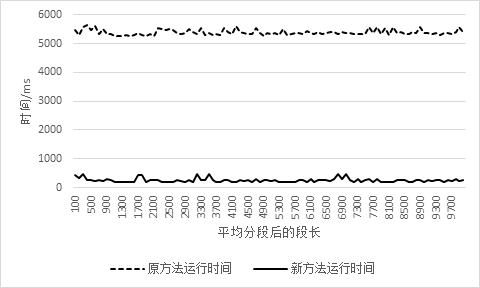
\includegraphics[width=0.65\textwidth]{figures/figure4x2}
	\caption{生产数据平均分段下两种方法的耗时情况}\label{fig:fig42}
\end{figure}

由图\ref{fig:fig42}可知,不论分段段长为多大,缓存第一次的计算结果的计算方式,运行总时间远远小于原来的计算方式。当时序数据数据量$N$很大时,假设分段后的段长为$n$,拟合多项式的次数为$k$,则在原计算方式中,计算长度为$n$的数据段拟合多项式的系数时,$(X^TX)^{-1}X^TY$的计算时间为
\begin{equation}
\begin{split}
T((X^TX)^{-1}X^T) &= T((X^TX)) + T(M^{-1}) + T(NX^T)  + T(PY)\\
                  &= \left ( k+1 \right )^2n + \left ( k+1 \right )^{3} + \left ( k+1 \right )^2n+\left ( k+1 \right )n \\
                  &= 2n(k+1)^2 + (k+1) ^3 + n(k+1) \\
                  &\approx 2n(k+1)^2 + n(k+1)
\end{split}
\end{equation}
其中,矩阵$M, N, P$分别代表前面的矩阵的计算结果。因为$k$与$n$相比,是比较小的值,而且在实验过程中,发现需要进行求逆操作的矩阵规模比较小,求逆所需要的时间比较少,所以将这部分的时间忽略。段数一共有$N/n$段,则总时间为
\begin{equation} \label{equ:equ410}
\begin{split}
T_1 &= N/n * (2n(k+1)^2 + n(k+1)) \\
 &= N(2(k+1)^2 + (k+1))
\end{split}
\end{equation}
对于将第一次的中间结果缓存下来的计算方法中,只在第一次,进行了全部的计算,之后的计算中,只进行了中间矩阵结果和$Y$矩阵的相乘计算,则其总时间为
\begin{equation}\label{equ:equ411}
\begin{split}
T_2 &= 2n(k+1)^2 + (k+1) ^3 + n(k+1) + n(k+1)*(N/n-1) \\
&\approx N(k+1)
\end{split}
\end{equation}
由式子\ref{equ:equ410}和\ref{equ:equ411}可看出,将中间结果缓存的方法,计算复杂度更低,计算时间更短。而且,其计算时间与段长$n$没有关系,所以在图\ref{fig:fig42}中,无论段长为多少,两种方法的运行时间基本不变。

%%下一步写周期非平均分段,非周期的平均分段
当对周期时间采样的时序数据进行非平均分段后再进行多项式拟合时,此时的分段长度不再全部相同。此时,依然建立缓存区,缓存区存储不同长度的数据段对应的中间矩阵结果$(X^TX)^{-1}X^T$。当计算当前段的多项式系数时,先在缓存区中进行查找当前段长对应的中间矩阵结果,若有,直接使用,否则,计算出该矩阵结果并缓存起来供下次使用。为了验证该方法的加速效果,使用实际生产数据的前$1,000,000$数据进行实验,其中不平均分段算法采用自底向上算法,由不同的分段误差值可以得到不同的分段数目,实验结果如图\ref{fig:fig43}所示。从图中可以看出,在不平均分段的情况下,当分段数目很少时,原方法与新的计算方法的运行时间基本相同,没有起到加速效果,而随着分段数量的增加,新方法的运行时间相比于原方法迅速减少,分段数目越多,运行时间越少,加速效果越好,直至达到一个平稳的状态。

\begin{figure}[htb]
	\centering
	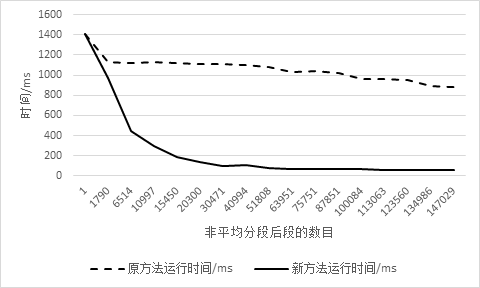
\includegraphics[width=0.65\textwidth]{figures/figure4x3}
	\caption{生产数据非平均分段下两种方法的耗时情况}\label{fig:fig43}
\end{figure}

\subsection{非周期时间采样的时序数据}
非周期时间采样的时序数据,其时刻序号不再是等差递增,而只是一个递增的无序序列,此时,为了简化计算,假设一段时序数据的时间戳为$t_1,t_2,...,t_n$,则将时刻序号中的第一项的值$x_1$记作$1$,第$i$项的值$x_i$记作$x_1 + t_i-t_1$。此时,对时序数据进行平均分段,虽然每段长度一样,但是每个时序段的时刻序号是不相同的。此时,再将第一次计算的中间矩阵结果缓存起来,下次去缓存中查找时,应该通过当前的时序数据段的时刻序号来进行查找,而不再是通过段长查找。其缓存结果如图\ref{fig:fig451}所示,通过查找时刻序号$T$来查找中间矩阵结果。为了验证这种情况下的加速效果,用UCI数据库中一个非周期时间采集的的关于人体运动的传感器数据集\upcite{GaitData}来进行实验,结果如图\ref{fig:fig44}所示。由图中可知,对非周期时间采样的时序数据的压缩采用缓存的方法,虽然其加速比不如周期时间采样的时序数据的加速比,仍能起到较好加速效果,加速比在$5$x$\sim 9$x之间。

\begin{figure}[htb]
	\centering
	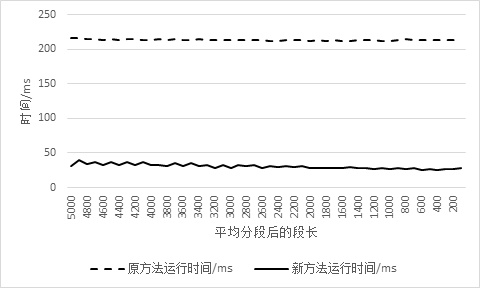
\includegraphics[width=0.65\textwidth]{figures/figure4x4}
	\caption{人体运动数据平均分段下两种方法的耗时情况}\label{fig:fig44}
\end{figure}

如果对非周期时间采集的时序数据进行非平均分段,其包含两个不同的因素,一是段长,二是时刻序号,相同的段长时刻序号也不一定相同。如果采用缓存的方法,缓存需要设计为二级缓存,缓存结构如图\ref{fig:fig452}所示。这种情况下的加速效果不是特别理想,因此此处只给出思路。首先查找当前段长,然后再查找段长对应的时刻序号,最后得到是否已经有中间计算结果。

\begin{figure}[htbp]
	\centering                                      %居中
	\subfigure[平均分段]{              %第一张子图
		\begin{minipage}{6cm}
			\label{fig:fig451}
			\centering                              %子图居中
			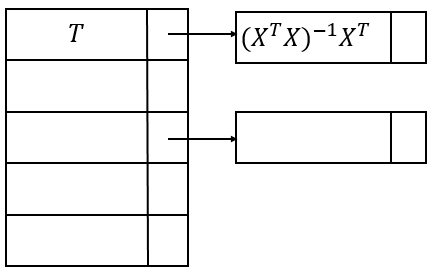
\includegraphics[width=0.7\textwidth]{figures/figure4x51}   %以pic.jpg的0.5倍大小输出
		\end{minipage}
	}
	\subfigure[非平均分段]{                  %第二张子图
		\begin{minipage}{9cm}
			\label{fig:fig452}
			\centering                                  %子图居中
			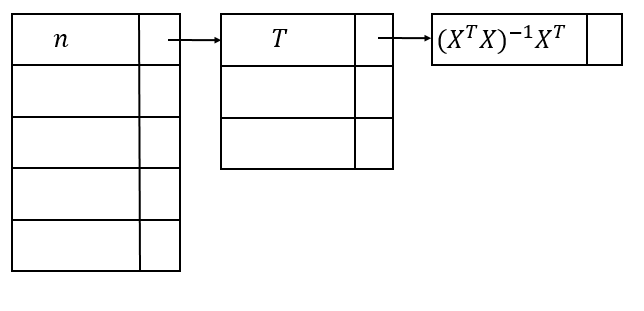
\includegraphics[width=0.7\textwidth]{figures/figure4x52}       %以pic.jpg的0.5倍大小输出
		\end{minipage}
	}\caption{非周期时间采样的时序数据所用缓存数据结构} %                     %大图名称
	\label{fig:fig45}                                       %图片引用标记
\end{figure}
%总结
这一小节主要分析了静态时序数据的压缩,在已知数据整体的情况下,对于周期时间采样的时序数据,进行平均分段和不平均分段的多项式拟合时,其加速方法及其效果。对于非周期时间采样的时序数据时,进行平均分段时,其多项式拟合的加速方法及其效果,以及采用非均匀分段时,其加速想法。下一小节分析在流式计算环境下,对于流式时序数据的压缩及其加速。

\section{流式时序数据压缩加速方法研究}
本节对流式时序数据进行压缩分析。在进行分段时,不均匀分段比均匀分段更能体现数据本身的特性,有利于保留原始序列的主体特征。所以,本文选择对原始数据进行不均匀分段的多项式拟合操作进行数据的压缩。

因为流式数据的特点,压缩过程是动态的,需要进行在线的压缩,所以选择滑动窗口算法来进行分段。该过程如下。假设给定误差值为$\varepsilon $,当前窗口内的已有点为
$\left \{ \left ( x_{1},y_{1} \right ),\left ( x_{2},y_{2} \right ),...,\left ( x_{m},y_{m} \right ) \right \}$,
拟合后的多项式函数为$f_{m}\left ( x \right )$,则必有
\begin{equation}\sum_{i=1}^{m}\left ( f_{m}\left ( x_{i} \right )-y_{i} \right )^{2}\leq m*\varepsilon \end{equation}
当新的数据点$\left ( x_{m+1},y_{m+1} \right )$到达窗口内后,首先计算当前拟合函数$f_{m}\left ( x \right )$是否可以在误差值$\varepsilon $下拟合点
$\left \{ \left ( x_{1},y_{1} \right ),\left ( x_{2},y_{2} \right ),...,\left ( x_{m+1},y_{m+1} \right ) \right \}$。
若\begin{equation}\sum_{i=1}^{m+1}\left ( f_{m}\left ( x_{i} \right )-y_{i} \right )^{2}\leq (m+1)*\varepsilon \end{equation}
则\begin{equation}f_{m+1}\left ( x \right ) = f_{m}\left ( x \right )\end{equation}否则,需要对当前窗口内$m+1$个点进行新的多项式拟合。重复此过程直至当前段已达到最大数量,再多一个数据点后拟合后的误差值大于$\varepsilon $,此时,窗口内的数据点分为一个数据段,窗口重新开始接收新的数据作为新的一段。该过程表达如算法\ref{alg:PRRA}所示。

\begin{algorithm}
	\KwIn{Streaming time-series data}
	
	\KwOut{the polynomial coefficient after fitting}
	
	%\SetVline
	
	Let $k$ be the degree of polynomials\;
	Let $\varepsilon$ be the predefined error bound\;
	$temp\_seg = \phi$\;
	\While{input($x$, $y$)}{
		$temp\_seg = temp\_seg \cup {(x, y)}$\;
		\If{Length(temp\_seg)$ = k+1$}{
			$temp\_A = calculatePolynomial(temp\_seg, k)$\;
			$A = temp\_A$\;
			$seg = temp\_seg$\;
		}
		\Else{
			\If{Length($temp\_seg$) $> k+1$}{
				\If{calculateError($temp\_seg, temp\_A$) $>\varepsilon$}{
					$temp\_A = calculatePolynomial(temp\_seg, k)$\;
					\If{calculateError($temp\_seg$, $temp\_A$) $> \varepsilon$}{
						$save(A, seg)$\;
						$temp\_seg = \{(x, y)\}$\;
					}
					\Else{
						$A = temp\_A$\;
						$seg = temp\_seg$\;
					}
				}
			}
		}
	}
	\caption{流式时序数据的在线多项式拟合算法}
	\label{alg:PRRA}
\end{algorithm}

用多项式拟合来压缩时序数据的过程,就是得到多项式系数的过程。由以上内容可知,每来一个数据点时基本都要进行一次系数矩阵的计算,而且计算过程需要进行矩阵的乘法和求逆的运算,矩阵的规模可以达到当前数据段段长的平方。当窗口内的数据量很大时,这将是一笔巨大的计算时间开销。时序数据分为周期时间采集的与非周期时间采集的数据。针对这两类不同时刻序号的时序数据,对其压缩过程的加速也是不同的。

\subsection{周期时间采样的时序数据}
由上节内容可知,周期时间采集的时序数据的时刻序号$T$为$1,2,3...$,此时,式子\ref{eq:411}中的$x_i = i$。此时,由式子\ref{eq:411}和\ref{eq:412}可知,如果两个时序数据的序列的段长相同,则其时刻序号相同,矩阵$X$是相同的,从而$(X^TX)^{-1}X^T$的矩阵结果是相同的。而在对时序数据进行在线压缩时,滑动窗口内的数据是依次增加的,所以,压缩后任意不同两段的时序数据在压缩的过程中,前期长度一样的时候,其$X$是一样的,则中间矩阵计算结果$(X^TX)^{-1}X^T$也是一样的。而且,假设经过压缩后有任意两段时序数据,则长度较短的一段的时刻序号必定是长度较长的一段的时刻序号的前缀。则在计算较短段长的时序数据段的过程中,其计算得到的$(X^TX)^{-1}X^T$中间结果必定是计算较长段长时序数据段的过程中需要的中间结果的一部分。而矩阵的计算是十分消耗时间的,假如建立一个缓存区域,将已经计算过的矩阵结果缓存起来,在下一次计算的时候,在缓存区域查找是否已经有计算结果,如果有,可以避免进一步的计算,可以减少计算时间,进行加速。所以,对于周期时间采样的时序数据,可以通过空间换时间的思想,重复利用矩阵的中间计算结果,来减少计算时间。

\subsubsection{建立缓存}
段长为$n$的时序数据的时刻序号$x_1,x_2,x_3,...,x_n$为$1,2,3,...,n$,则段长为$n$的时序数据进行多项式拟合,求解拟合多项式系数矩阵时,式子\ref{eq:412}中的$(X^TX)^{-1}X^T$的结果值是一样的。所以,对于唯一的段长值$n$,可以唯一确定值$(X^TX)^{-1}X^T$。因此,如果在计算过程中,对于当前长度为$n$的时序数据段,首先去缓存查找是否有$n$对应的$(X^TX)^{-1}X^T$计算结果,如果有,直接使用该结果;如果没有,计算出矩阵结果,并且将该结果存储在缓存区域,下一次即可不需计算直接使用。此时,在对流式时序数据进行多项式拟合时,对于不同段长的数据段的$(X^TX)^{-1}X^T$计算只需要进行一次,而在之后的运算中,由原来三次的矩阵乘法运算和一次矩阵求逆运算减少到只需要一次矩阵乘法计算,大大地减少了计算步骤,提高了计算效率。

$(X^TX)^{-1}X^T$的计算结果是一个$(k+1)*n$的矩阵,其中,$k$是拟合多项式的次数,则$k+1$是多项式的系数的个数,$n$是被拟合的时序数据段的段长。假设$k = 6$,$n = i$,元素数据类型为$double$型,每个元素占$8$字节,则一个矩阵占用空间为$(6+1)*i*8 = 56iB$, 则假设最长时序数据段段长为$N$,则所占的内存空间为
\begin{equation}
\sum_{i=1}^{N}56i = 28N(N+1) B
\end{equation}
如果缓存空间大小为$128MB$,则$N \approx 2189$,所以可以缓存的矩阵计算结果的时序数据的长度可达$2189$,所以使用存储矩阵的方法来减少计算时间进行拟合加速是可行的。

\subsubsection{缓存结构}
由上节内容可知,确定的时序数据段段长$n$对应的中间结果是唯一的,所以缓存可以采用哈希表表示,数据结构如图\ref{fig:fig41}所示。

\begin{figure}[htb]
	\centering
	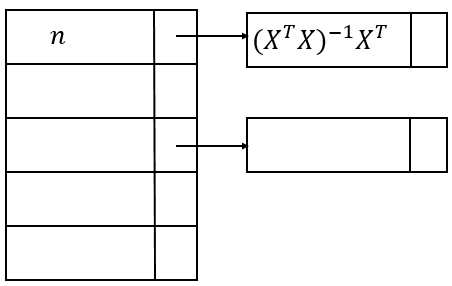
\includegraphics[width=0.35\textwidth]{figures/figure4x1}
	\caption{缓存区域的数据结构}\label{fig:fig41}
\end{figure}

其中,拟合的时序数据的段长$n$为关键字$key$,该段长对应的中间结果矩阵值$(X^TX)^{-1}X^T$为$key$对应的$value$。$key$的存储以数组形式存储,所以查找速度很快,相比于计算时间几乎不消耗多余时间。

\subsection{非周期时间采样的时序数据}
非周期时间采样的时序数据,如果建立缓存,因为段长和时刻序号都不相同,通过实验发现加速效果很差,而且还浪费缓存内存与查找时间,所以,这种情况下不再使用缓存的方法。

假设当前窗口内的数据段为${\left \{ (x_1,y_1),(x_2,y_2),..., (x_n,y_n)\right \}}$,则其多项式系数矩阵$A=(X^TX)^{-1}X^TY$。可以得到,
\begin{equation}
X^TX = \begin{bmatrix}
n&{\sum_{i=1}^n \limits x_i}& \cdots & {\sum_{i=1}^n \limits x_i^k} \\
{\sum_{i=1}^n \limits x_i}&{\sum_{i=1}^n \limits x_i^2}& \cdots & {\sum_{i=1}^n \limits x_i^{k+1}}\\
\vdots & \vdots & \ddots & \vdots \\
{\sum_{i=1}^n \limits x_i^k}&{\sum_{i=1}^n \limits x_i^{k+1}}& \cdots & {\sum_{i=1}^n \limits x_i^{2*k}}
\end{bmatrix}
\end{equation}

\begin{equation}
X^TY = \begin{bmatrix}
{\sum_{i=1}^n \limits y_i} \\
{\sum_{i=1}^n \limits x_iy_i} \\
\vdots \\
{\sum_{i=1}^n \limits x_i^ky_i}
\end{bmatrix}
\end{equation}
当窗口内新来一个数据点$(x_{n+1},y_{n+1})$时,当前被拟合的数据段为 $\{(x_1, y_1), (x_2, y_2), ...,$ $(x_n, y_n), (x_{n+1}, y_{n+1})\}$,多项式的系数矩阵 $A' = (X'^TX')^{-1}X'^TY'$,在这个式子中,有
\begin{equation} \label{equ:equ419}
\begin{split}
X'^TX' &= \begin{bmatrix}
{n+1}&{\sum_{i=1}^{n+1} \limits x_i}& \cdots & {\sum_{i=1}^{n+1} \limits x_i^k} \\
{\sum_{i=1}^{n+1} \limits x_i}&{\sum_{i=1}^{n+1} \limits x_i^2}& \cdots & {\sum_{i=1}^{n+1} \limits x_i^{k+1}}\\
\vdots & \vdots & \ddots & \vdots \\
{\sum_{i=1}^{n+1} \limits x_i^k}&{\sum_{i=1}^{n+1} \limits x_i^{k+1}}& \cdots & {\sum_{i=1}^{n+1} \limits x_i^{2*k}}
\end{bmatrix} \\
&=
\begin{bmatrix}
n&{\sum_{i=1}^n \limits x_i}& \cdots & {\sum_{i=1}^n \limits x_i^k} \\
{\sum_{i=1}^n \limits x_i}&{\sum_{i=1}^n \limits x_i^2}& \cdots & {\sum_{i=1}^n \limits x_i^{k+1}}\\
\vdots & \vdots & \ddots & \vdots \\
{\sum_{i=1}^n \limits x_i^k}&{\sum_{i=1}^n \limits x_i^{k+1}}& \cdots & {\sum_{i=1}^n \limits x_i^{2*k}}
\end{bmatrix}
+ 
\begin{bmatrix}
1& x_{n+1} & \cdots &  x_{n+1}^k \\
x_{n+1}& x_{n+1}^2 & \cdots &  x_{n+1}^{k+1} \\
\vdots & \vdots & \ddots & \vdots \\
x_{n+1}^k& x_{n+1}^{k+1} & \cdots &  x_{n+1}^{2*k}
\end{bmatrix} \\
&=
X^TX +
\begin{bmatrix}
1& x_{n+1} & \cdots &  x_{n+1}^k \\
x_{n+1}& x_{n+1}^2 & \cdots &  x_{n+1}^{k+1} \\
\vdots & \vdots & \ddots & \vdots \\
x_{n+1}^k& x_{n+1}^{k+1} & \cdots &  x_{n+1}^{2*k}
\end{bmatrix}
\end{split} 
\end{equation}
由式子\ref{equ:equ419}可知,$X'^TX'$的结果由两部分组成,一部分是之前计算过的结果$X^TX$,是不变的部分,一部分只与新来的数据点的时刻值$X_{n+1}$有关,是可变的部分。所以每次做计算时,将$X^TX$的结果临时存储一下,那么进行下次拟合计算的时候,只需要计算可变部分的结果,然后将不变部分与可变部分做矩阵相加即可得到$X'^TX'$的结果。这次的结果依旧可以作为临时变量存起来,作为下次计算结果的一部分。该方法采取了增量计算的思想,每一批计算的结果是由之前数据的结果与增量的数据的结果得到的,即每次新来一个数据点后,只计算该数据点带来的影响变化,并将这个变化应用到之前的结果上。这种方法可以减少一部分的数据计算,进而进行计算过程的加速。同理,在计算$X'^TY'$时,有
\begin{equation}
\begin{split}
 X'^TY' &=
\begin{bmatrix}
{\sum_{i=1}^{n+1} \limits y_i} \\
{\sum_{i=1}^{n+1} \limits x_iy_i} \\
\vdots \\
{\sum_{i=1}^{n+1} \limits x_i^ky_i}
\end{bmatrix} \\
&=
\begin{bmatrix}
{\sum_{i=1}^n \limits y_i} \\
{\sum_{i=1}^n \limits x_iy_i} \\
\vdots \\
{\sum_{i=1}^n \limits x_i^ky_i}
\end{bmatrix}
+
\begin{bmatrix}
y_{n+1}\\
x_{n+1}y_{n+1}\\
\vdots \\
x_{n+1}^ky_{n+1}
\end{bmatrix}\\
&=
X^TY + \begin{bmatrix}
y_{n+1}\\
x_{n+1}y_{n+1}\\
\vdots \\
x_{n+1}^ky_{n+1}
\end{bmatrix}
\end{split}
\end{equation}

因此,$X'^TY'$部分的计算,依旧可以采用增量计算的思想,通过将$X^TY$的结果与计算新来的数据点$(x_{n+1},y_{y+1})$得到的可变部分的结果相加得到。从上面这些分析可知,在流式环境下,当对非周期时间采样的时序数据进行压缩时,可以在计算过程中采用增量计算的方法减少计算量。等新来一个数据点时,上一次计算结果可以重复使用,而这次的结算结果,又可以作为下一次计算的部分结果使用。每一次只需要计算新来数据点带来的可变部分的结果即可。而且由式子可知,这种方法不需要缓存滑动窗口内的数据点为${\left \{ (x_1,y_1),(x_2,y_2),..., (x_n,y_n)\right \}}$,只需要存储每次的$X^TX$与$X^TY$的结果即可。
\section{本章小结}
本章介绍了对流式时序数据进行在线压缩的过程。针对数据的在线压缩选择了滑动窗口的算法,并且给出了多项式拟合的伪代码和计算其系数的过程。针对周期时间采样的时序数据的时刻序号的特点,设计了一种缓存的方式,以空间换时间,来减少计算过程中关于矩阵的计算,减少了计算时间,提高了计算效率,保证了流式数据计算的实时性。而对于非周期时间采样的时序数据,分析了其计算过程,提出了一种增量计算的方法,减少了数据的计算量,对拟合进行了加速。